% Options for packages loaded elsewhere
% Options for packages loaded elsewhere
\PassOptionsToPackage{unicode}{hyperref}
\PassOptionsToPackage{hyphens}{url}
\PassOptionsToPackage{dvipsnames,svgnames,x11names}{xcolor}
%
\documentclass[
  11pt,
  letterpaper,
  DIV=11,
  numbers=noendperiod]{scrartcl}
\usepackage{xcolor}
\usepackage{amsmath,amssymb}
\setcounter{secnumdepth}{5}
\usepackage{iftex}
\ifPDFTeX
  \usepackage[T1]{fontenc}
  \usepackage[utf8]{inputenc}
  \usepackage{textcomp} % provide euro and other symbols
\else % if luatex or xetex
  \usepackage{unicode-math} % this also loads fontspec
  \defaultfontfeatures{Scale=MatchLowercase}
  \defaultfontfeatures[\rmfamily]{Ligatures=TeX,Scale=1}
\fi
\usepackage{lmodern}
\ifPDFTeX\else
  % xetex/luatex font selection
\fi
% Use upquote if available, for straight quotes in verbatim environments
\IfFileExists{upquote.sty}{\usepackage{upquote}}{}
\IfFileExists{microtype.sty}{% use microtype if available
  \usepackage[]{microtype}
  \UseMicrotypeSet[protrusion]{basicmath} % disable protrusion for tt fonts
}{}
% Make \paragraph and \subparagraph free-standing
\makeatletter
\ifx\paragraph\undefined\else
  \let\oldparagraph\paragraph
  \renewcommand{\paragraph}{
    \@ifstar
      \xxxParagraphStar
      \xxxParagraphNoStar
  }
  \newcommand{\xxxParagraphStar}[1]{\oldparagraph*{#1}\mbox{}}
  \newcommand{\xxxParagraphNoStar}[1]{\oldparagraph{#1}\mbox{}}
\fi
\ifx\subparagraph\undefined\else
  \let\oldsubparagraph\subparagraph
  \renewcommand{\subparagraph}{
    \@ifstar
      \xxxSubParagraphStar
      \xxxSubParagraphNoStar
  }
  \newcommand{\xxxSubParagraphStar}[1]{\oldsubparagraph*{#1}\mbox{}}
  \newcommand{\xxxSubParagraphNoStar}[1]{\oldsubparagraph{#1}\mbox{}}
\fi
\makeatother


\usepackage{longtable,booktabs,array}
\usepackage{calc} % for calculating minipage widths
% Correct order of tables after \paragraph or \subparagraph
\usepackage{etoolbox}
\makeatletter
\patchcmd\longtable{\par}{\if@noskipsec\mbox{}\fi\par}{}{}
\makeatother
% Allow footnotes in longtable head/foot
\IfFileExists{footnotehyper.sty}{\usepackage{footnotehyper}}{\usepackage{footnote}}
\makesavenoteenv{longtable}
\usepackage{graphicx}
\makeatletter
\newsavebox\pandoc@box
\newcommand*\pandocbounded[1]{% scales image to fit in text height/width
  \sbox\pandoc@box{#1}%
  \Gscale@div\@tempa{\textheight}{\dimexpr\ht\pandoc@box+\dp\pandoc@box\relax}%
  \Gscale@div\@tempb{\linewidth}{\wd\pandoc@box}%
  \ifdim\@tempb\p@<\@tempa\p@\let\@tempa\@tempb\fi% select the smaller of both
  \ifdim\@tempa\p@<\p@\scalebox{\@tempa}{\usebox\pandoc@box}%
  \else\usebox{\pandoc@box}%
  \fi%
}
% Set default figure placement to htbp
\def\fps@figure{htbp}
\makeatother


% definitions for citeproc citations
\NewDocumentCommand\citeproctext{}{}
\NewDocumentCommand\citeproc{mm}{%
  \begingroup\def\citeproctext{#2}\cite{#1}\endgroup}
\makeatletter
 % allow citations to break across lines
 \let\@cite@ofmt\@firstofone
 % avoid brackets around text for \cite:
 \def\@biblabel#1{}
 \def\@cite#1#2{{#1\if@tempswa , #2\fi}}
\makeatother
\newlength{\cslhangindent}
\setlength{\cslhangindent}{1.5em}
\newlength{\csllabelwidth}
\setlength{\csllabelwidth}{3em}
\newenvironment{CSLReferences}[2] % #1 hanging-indent, #2 entry-spacing
 {\begin{list}{}{%
  \setlength{\itemindent}{0pt}
  \setlength{\leftmargin}{0pt}
  \setlength{\parsep}{0pt}
  % turn on hanging indent if param 1 is 1
  \ifodd #1
   \setlength{\leftmargin}{\cslhangindent}
   \setlength{\itemindent}{-1\cslhangindent}
  \fi
  % set entry spacing
  \setlength{\itemsep}{#2\baselineskip}}}
 {\end{list}}
\usepackage{calc}
\newcommand{\CSLBlock}[1]{\hfill\break\parbox[t]{\linewidth}{\strut\ignorespaces#1\strut}}
\newcommand{\CSLLeftMargin}[1]{\parbox[t]{\csllabelwidth}{\strut#1\strut}}
\newcommand{\CSLRightInline}[1]{\parbox[t]{\linewidth - \csllabelwidth}{\strut#1\strut}}
\newcommand{\CSLIndent}[1]{\hspace{\cslhangindent}#1}



\setlength{\emergencystretch}{3em} % prevent overfull lines

\providecommand{\tightlist}{%
  \setlength{\itemsep}{0pt}\setlength{\parskip}{0pt}}



 


\usepackage{caption}
\captionsetup{font=small, labelfont=bf}
\setlength{\parindent}{0pt}
\setlength{\parskip}{1.25ex}
\KOMAoption{captions}{tableheading}
\makeatletter
\@ifpackageloaded{caption}{}{\usepackage{caption}}
\AtBeginDocument{%
\ifdefined\contentsname
  \renewcommand*\contentsname{Table of contents}
\else
  \newcommand\contentsname{Table of contents}
\fi
\ifdefined\listfigurename
  \renewcommand*\listfigurename{List of Figures}
\else
  \newcommand\listfigurename{List of Figures}
\fi
\ifdefined\listtablename
  \renewcommand*\listtablename{List of Tables}
\else
  \newcommand\listtablename{List of Tables}
\fi
\ifdefined\figurename
  \renewcommand*\figurename{Figure}
\else
  \newcommand\figurename{Figure}
\fi
\ifdefined\tablename
  \renewcommand*\tablename{Table}
\else
  \newcommand\tablename{Table}
\fi
}
\@ifpackageloaded{float}{}{\usepackage{float}}
\floatstyle{ruled}
\@ifundefined{c@chapter}{\newfloat{codelisting}{h}{lop}}{\newfloat{codelisting}{h}{lop}[chapter]}
\floatname{codelisting}{Listing}
\newcommand*\listoflistings{\listof{codelisting}{List of Listings}}
\makeatother
\makeatletter
\makeatother
\makeatletter
\@ifpackageloaded{caption}{}{\usepackage{caption}}
\@ifpackageloaded{subcaption}{}{\usepackage{subcaption}}
\makeatother
\usepackage{bookmark}
\IfFileExists{xurl.sty}{\usepackage{xurl}}{} % add URL line breaks if available
\urlstyle{same}
\hypersetup{
  pdftitle={(Report) Image statistic encoding between regions of the visual cortex},
  pdfauthor={Al Xin},
  colorlinks=true,
  linkcolor={blue},
  filecolor={Maroon},
  citecolor={Blue},
  urlcolor={Blue},
  pdfcreator={LaTeX via pandoc}}


\title{(Report) Image statistic encoding between regions of the visual
cortex}
\author{\small Al Xin}
\date{Aug 12, 2026}
\begin{document}
\maketitle


\section{Introduction}\label{introduction}

\subsection{Motivation}\label{motivation}

Later stages of the visual cortex are thought to contain neurons
selective for progressively higher-level visual features. One approach
to characterize the relevant visual features for each layer is through
characterizing responses to visual textures with known image statistics.
Visual textures can be loosely described as approximately homogeneous
images with repeating but randomized elements, e.g., images of sand,
tree bark, granite, or honeycomb. Here, image statistics refer to
\(N\)th-order empirical densities of pixels. First order statistics
include, for example, luminance correlations at a given distance.

Portilla and Simoncelli (2000)
{[}\citeproc{ref-portilla_parametric_2000}{1}{]} developed a parametric
texture model that, given a seed image of a visual texture, generates
new samples matched to the original's image statistics. The parametric
model can be adjusted to include higher-order statistics, which Portilla
and Simoncelli describe as V1-like. Matching V1-like correlations
produces more coherent \emph{naturalistic} structure. Example noisy (no
V1-like statistic matching) and naturalistic images can be seen in
Figure~\ref{fig-textures}. Freeman et al.~(2013) found that this
distinction may be relevant for functionally characterizing V2, finding
that V2 neurons tend to be more selective for naturalistic textures
{[}\citeproc{ref-freeman_functional_2013}{2}{]}.

\begin{figure}

\centering{

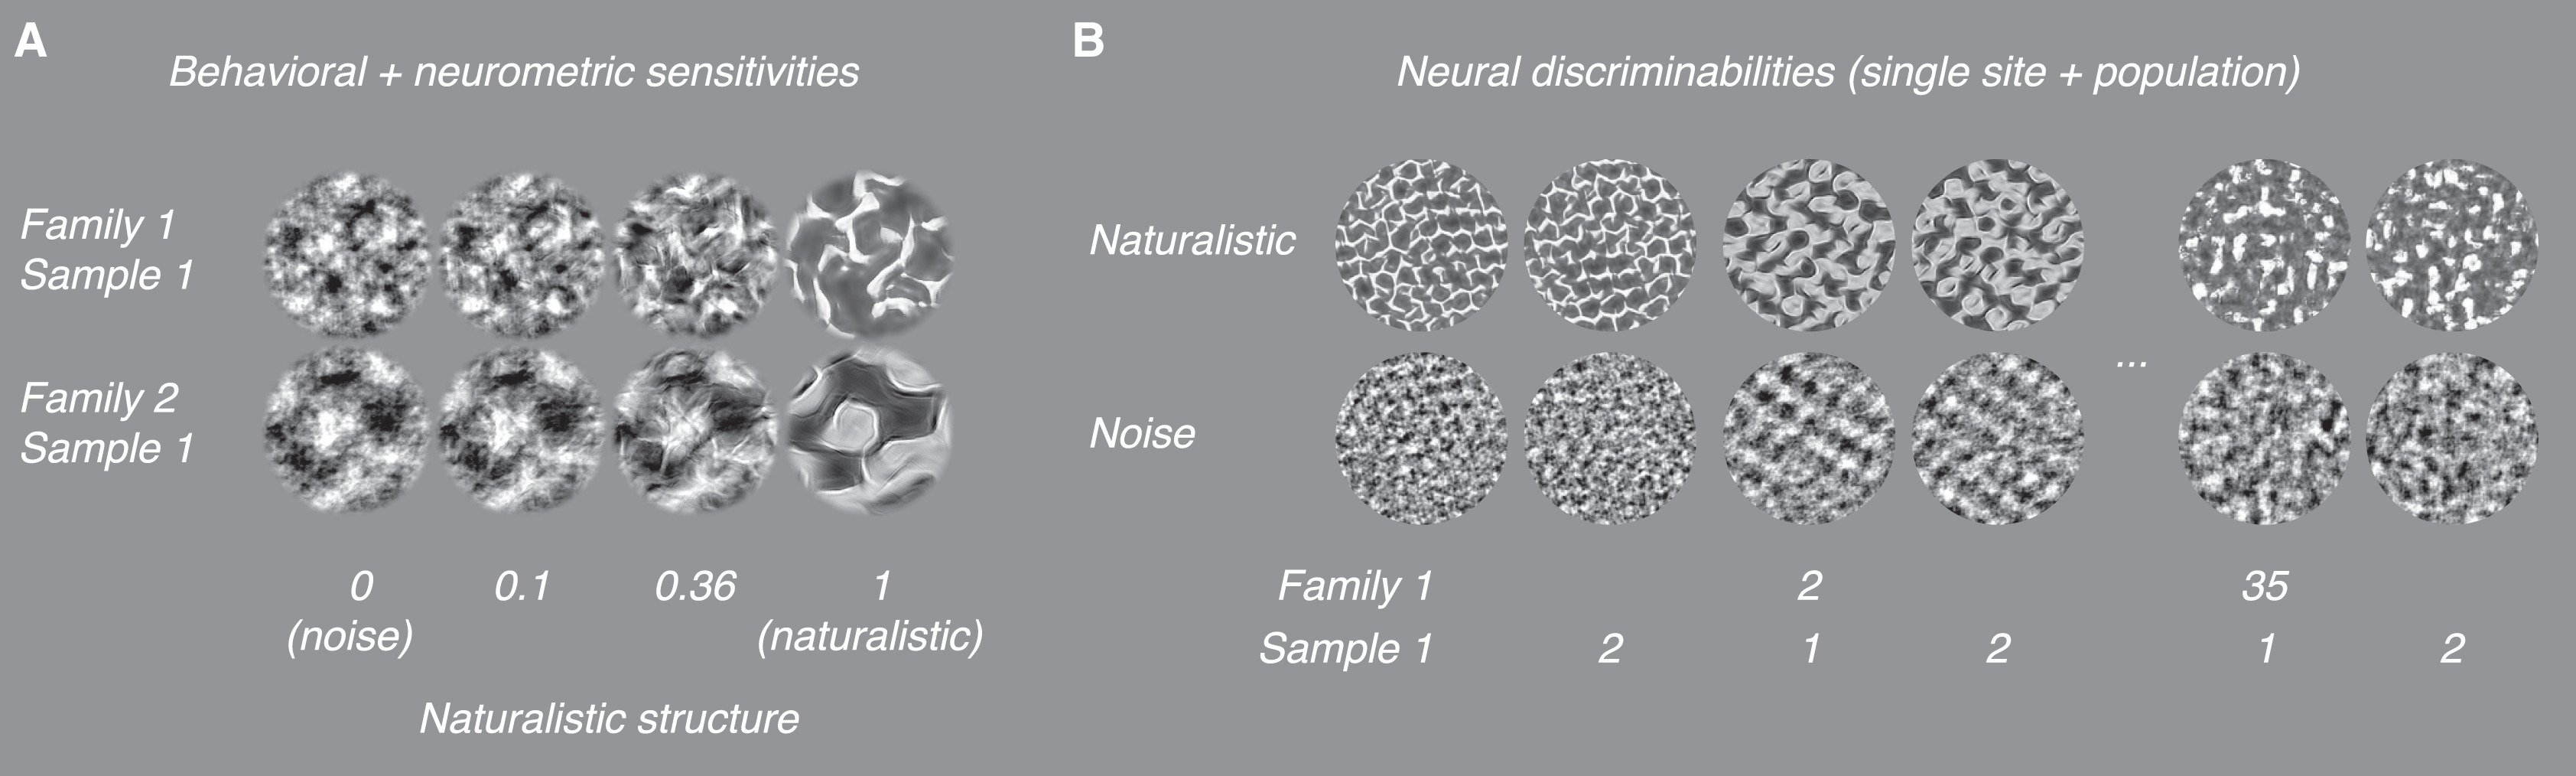
\includegraphics[width=0.9\linewidth,height=\textheight,keepaspectratio]{../img/lee2024-fig01.jpg}

}

\caption{\label{fig-textures}(A) Examples of samples generated with
varying levels of naturalistic structure. (B) Families of samples
generated from different seed images.}

\end{figure}%

My ADA will focus on further characterizing how image statistics may be
represented/transformed in V1, V2, V4, and IT, using data collected by
Lee et al.~(2024) {[}\citeproc{ref-lee_developmentally_2024}{3}{]}. V4
and IT are not usually recorded for visual texture stimuli. Each family
contains samples that are matched to the same statistics, but each
sample is unique at a pixel level. Thus, if higher layers are selective
for certain higher level aggregated image statistics, we expect that
they will lose selectivity for the differences between samples.

\subsection{Data}\label{data}

I sourced data from Gerick Lee et al.~(2024), who collected longitudinal
and inter-region neural responses to visual texture stimuli (available
on \href{https://zenodo.org/records/10888270}{Zenodo})
{[}\citeproc{ref-lee_developmentally_2024}{3}{]}. Lee et al.~recorded
from 6 macaques with two arrays each, targeting V1, V2, V4, and IT. Lee
et al.~reported the multi-unit activations; the spiking/raw timing data
are not available. Lee et al.~generated 15 samples of noisy and
naturalistic images from 35 families (\(15 \times 35 \times 2\) unique
images), where each family corresponded to a different original seed
image. The parameters fed into the PS model are lost, but the images
presented to the monkeys may be available.

\subsection{Expected results}\label{expected-results}

We expect to find better between-group discrimination in V2 and V4
better within-group discrimination in V1, i.e., more separation between
unique samples with the same visual statistics. That is, later visual
regions better encode relevant group-level visual statistics at the cost
of distinctively encoding individual instances of textures with the same
statistics (see Figure~\ref{fig-intro}). This effect is likely only
visible in population level metrics or decoding strategies considering
the relative size of the receptive fields. Previously, Ziemba et
al.~(2016) performed a similar analysis on recordings from V1 and V2
{[}\citeproc{ref-ziemba_selectivity_2016}{4}{]}. With nested ANOVA,
Ziemba et al.~found larger between-family variance in V1 but smaller
within-family contribution to variance. Ziemba et al.~(2016) also found
better performance of a Poisson decoder on classifying samples in V1
(and families in V2). Furthermore, for IT, it is possible that both
between-family and within-family distance decreases as IT may not be
sensitive to the image statistics that distinguish the textures, a
pattern found in Gerick Lee's previous analysis
(Figure~\ref{fig-areadne2024}).

\begin{figure}

\centering{

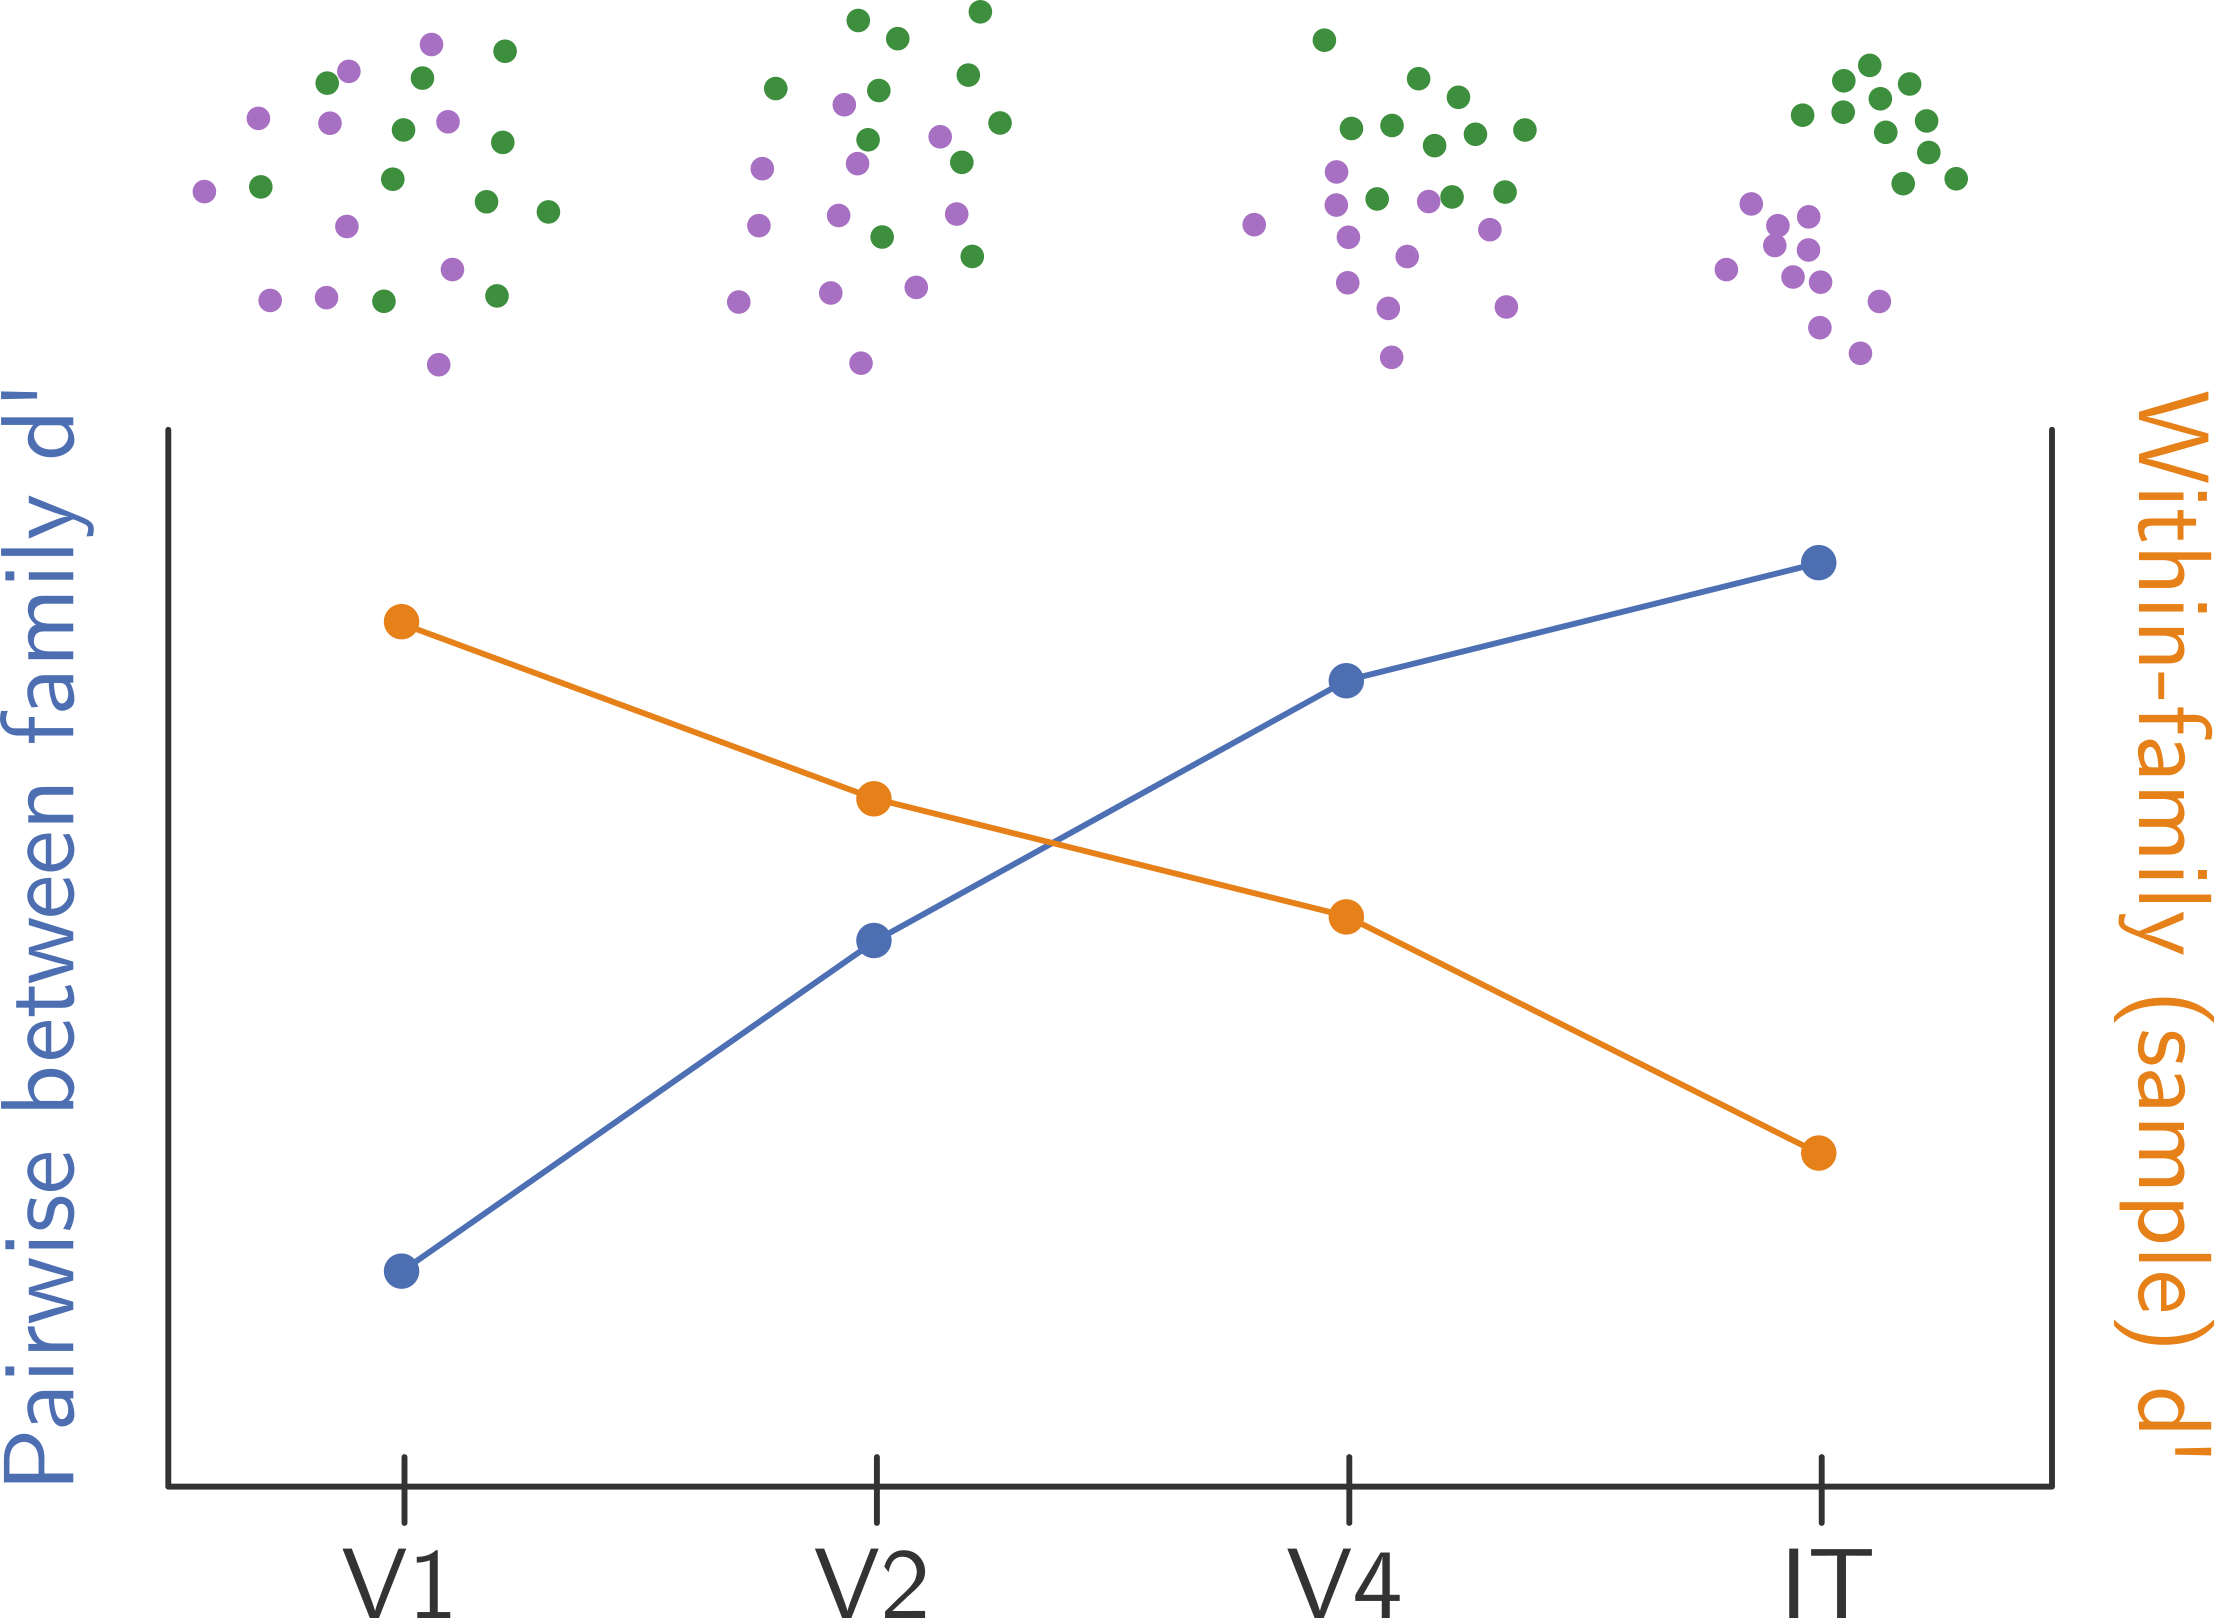
\includegraphics[width=0.6\linewidth,height=\textheight,keepaspectratio]{../img/proposed_results.png}

}

\caption{\label{fig-intro}(Top) A visual representation of two families
in some arbitrary 2D representation space. (Bottom) The distances
between families and between samples, with some arbitrary values for
each region.}

\end{figure}%

\begin{figure}

\centering{

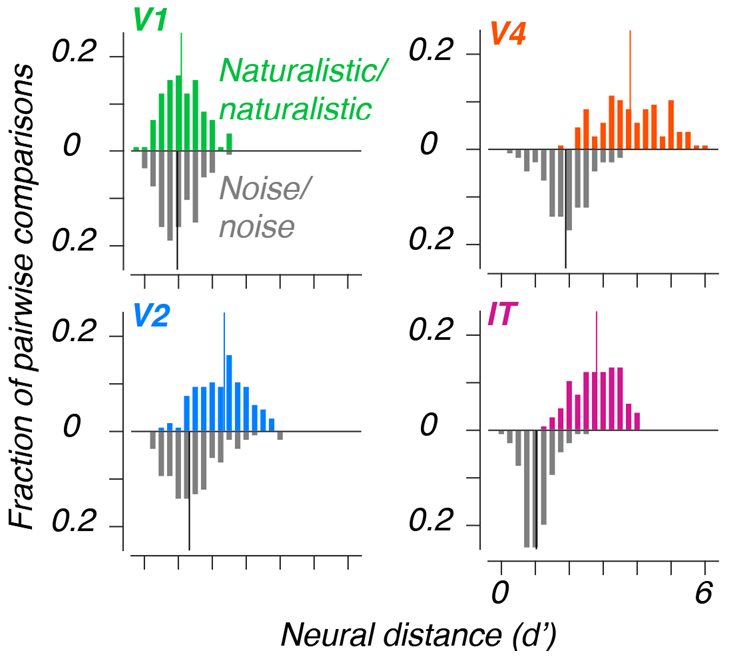
\includegraphics[width=0.4\linewidth,height=\textheight,keepaspectratio]{../../reports/img/lee2024-poster-1.png}

}

\caption{\label{fig-areadne2024}Histograms of pairwise comparisons, for
naturalistic-naturalistic comparisons (colored bars), and noise-noise
comparisons (gray). Lines depict medians. The figure was originally
vertical but I rearranged it, so the axes are consistent for all
quadrants.}

\end{figure}%

\subsection{Notes}\label{notes}

\begin{itemize}
\tightlist
\item
  Consecutive question marks (??) tag areas to follow up on.
\item
  Though the Lee et al.~paper and related literature describes textures
  without V1-like correlations as ``noise'', I often use the term
  ``noisy''.
\item
  For multivariate distance, I use Mahalanobis distance, indicated as
  \(d_M\)
\item
  The published data only includes multi-unit activations (MUAs) for
  each recording site.
\item
  Section~\ref{sec-data} mostly copies information from the previous
  report.
\end{itemize}

\section{Analysis plan}\label{analysis-plan}

To determine the between-family or between-sample separation within
regions, I will find the distribution of multivariate distance values
between pairwise comparisons. This approach will allow for visualization
of the median/mean pairwise distribution and the skew of the distances.

A multivariate distance value can be calculated with the typical
Mahalanobis distance formula, i.e., \[
d_M (\mathbf{x}, \mathbf{y}) = \sqrt{(\mathbf{x} - \mathbf{y})^\intercal \Sigma^{-1} (\mathbf{x} - \mathbf{y})},
\] where \(\mathbf{x}, \mathbf{y}\) correspond to the mean activity
vectors for each group, taken with respect to each site. The pooled
covariance matrix is the same as used in Hotelling's two-sample
statistic, derived as \[
\Sigma = 
\frac{(n_x - 1) \Sigma_x + (n_y - 1)\Sigma_y}{n_x + n_y - 2},
\] where \(\Sigma_x, \Sigma_y\) are the typical sample covariance
matrices for each distribution. \texttt{Rfast} contains functions
\texttt{Rfast::pooled.cov()} and \texttt{Rfast::spdinv()} to support
these calculations. For low trial numbers, the inverse covariance matrix
can be found with the regularized/shrinkage estimator from
\texttt{corpcor::invcov.shrink()}.

For between-family calculations, each family contains 90 trials (15
samples by 6 repetitions each). For between-sample distance
calculations, each sample only contains 6 repetitions. So, while
pairwise between-family calculations are straightforward, the
between-sample distances may need to be modified and explored more.

Jenelle proposed a randomized dichotomy procedure. Two groups of 7
sample IDs each (without replacement) will be selected. Because this is
not an even split of the available sample IDs, the procedure will
proceed as follows:

\begin{enumerate}
\def\labelenumi{\arabic{enumi}.}
\tightlist
\item
  Omit one of the 15 IDs (1, 2, \ldots, 15)
\item
  Take a random sample of the possible \(\binom{14}{7}\) combos of the
  remaining indices.
\item
  Find \(d_M\) between the two groups of seven samples (so 42 trials)
  each.
\item
  Repeat the above for each of the 15 IDs.
\end{enumerate}

Alternatively, we could still perform pairwise between-sample
calculations (with the regularized/shrinkage estimator) and discuss
trends visible within families.

\section{Data}\label{sec-data}

Monkeys were presented with textures generated from the PS parametric
texture model {[}\citeproc{ref-portilla_parametric_2000}{1}{]}, with
unique images created from 2 levels of coherence (noisy/naturalistic),
35 families (seed images), and 15 randomly generated samples from each
family. This produces 1050 unique images (\(35 \times 2 \times 15\)).
There are six repetitions of each image per session.

Lee et al.~recorded from 6 monkeys, each implanted with two 96-site Utah
arrays. Within a session, there were 6 repetitions of each of the
\(35 \times 15 \times 2 = 1050\) unique images, presented in blocks of 8
images (100 ms on, 100 ms off). The provided files aggregate recordings
by region, with the number of sites per region in Table~\ref{tbl-sites}.
For each of V1, V2, V4, and IT, there is at least one 96-electrode Utah
array. The published per-session data reflects simultaneously recorded
sites.

On M1, one array sat on the border between V1 and V2. For M3, the
authors could not reliably determine the location and labeled the region
as the foveal confluence (FC) of V1, V2 and V4, which I removed from my
analyses. Lee et al.~implanted IT arrays twice in M6, with the recording
at 221 weeks taken from the second implantation.

\begin{longtable}[]{@{}llllll@{}}
\caption{The array number is arbitrary. Monkey ID is in
parentheses.}\label{tbl-sites}\tabularnewline
\toprule\noalign{}
Region & Array 1 & Array 2 & Array 3 & Array 4 & Total \\
\midrule\noalign{}
\endfirsthead
\toprule\noalign{}
Region & Array 1 & Array 2 & Array 3 & Array 4 & Total \\
\midrule\noalign{}
\endhead
\bottomrule\noalign{}
\endlastfoot
V1 & 61 (M1) & 96 (M6) & & & 157 \\
V2 & 35 (M1) & 96 (M2) & & & 131 \\
V4 & 96 (M1) & 96 (M2) & 96 (M8) & & 288 \\
IT & 96 (M3) & 96 (M6) & 96 (M6) & 96 (M7) & 384 \\
\end{longtable}

\subsection{Behavioral discrimination between noisy and naturalistic
textures}\label{behavioral-discrimination-between-noisy-and-naturalistic-textures}

In addition to passive fixation recordings, Lee et al.~also measured
behavioral sensitivities with a four-choice oddity task. Monkeys were
shown 3 noisy distractors and 1 naturalistic target, with all four
images produced from the same family. The noisy distractors were unique
samples, i.e., not replicates of the same noisy image. The strength of
naturalistic structure in the target could be modified from 0
(statistically matched to noisy texture) to 1 (fully matches the
naturalistic structure statistics of the seed image). Of the 35 texture
families presented in passive fixation recordings, samples from only
five families were used in the behavioral task. The family IDs in the
behavioral task are included in the public MATLAB code. M8 only
underwent passive fixation recording and did not perform the four-choice
oddity task. M1, M2, and M3 performed the behavioral task prior to
recording while M6 and M7 performed the task after.

\section{Initial results}\label{initial-results}

\subsection{Between family
comparisons}\label{between-family-comparisons}

The trend in the results seem consistent with Gerick's poster (copied in
Figure~\ref{fig-areadne2024} for reference), with the center of the
histogram generally tending toward higher distances with higher visual
regions with the trend reversing in IT. Furthermore, while the
calculated distances tend to increase with more sub-sampled sites, the
overall trend in the distributions of the distance values is consistent
(Figure~\ref{fig-mahalanobis_sites}).

Figure~\ref{fig-dM_mu_var} contains plots for the difference in means
and inverse combined variance (averaged across sites). The term inverse
combined variance is used loosely, as it refers to the diagonal of the
\(\Sigma^{-1}\) in the Mahalanobis distance calculation. The inverse
combined variance tends to be lowest in V2, about even in V1 and V4, and
highest in IT. The difference in means tends to be about even in V1 and
V2 and smaller in V4 and IT.

(??) This is probably a bad approach to reasoning about the covariances
between the MUAs, since it would be easier to think about the original
un-inverted \(\Sigma\).

The greater \(d_M\) in V2 compared to V1 is not driven by the difference
in mean firing, as the V2 mean differences are smaller. Furthermore,
because the diagonal elements of \(\Sigma^{-1}\) are smaller in V2 than
V1, the overall \(d_M\) is probably being affected by larger
off-diagonal elements (i.e., smaller covariances between the sites). I
discarded these elements, so I need to redo these calculations if I
wanted to further investigate.

Similarly, the greater \(d_M\) in V4 compared to V2 is also not driven
by the difference in mean firing. The larger inverse combined variance
of V4 may account for the difference. That is, V4 firing has less
variance than V2.

The \(d_M\) in IT is smaller than V4 despite larger differences in mean
firing and larger inverse combined variance. Again, this points to
potential further exploration of the off-diagonal elements of
\(\Sigma^{-1}\).

Furthermore, the differences in the \(\Sigma^{-1}\) diagonal elements
suggest that z-scoring the firing averages may be needed.

\begin{figure}

\centering{

\pandocbounded{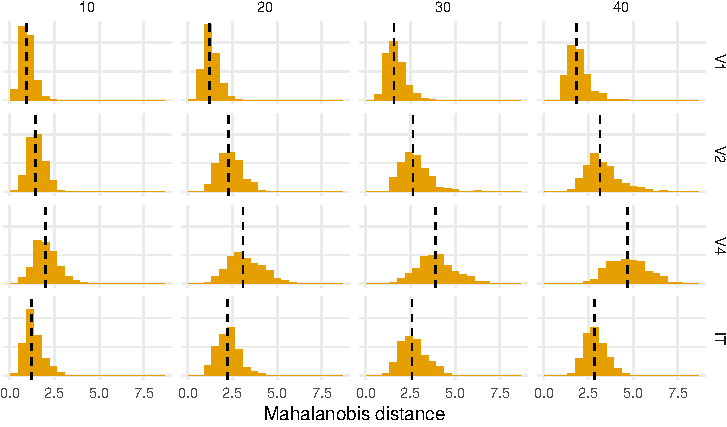
\includegraphics[keepaspectratio]{20260812_files/figure-pdf/fig-mahalanobis_sites-1.pdf}}

}

\caption{\label{fig-mahalanobis_sites}Histogram of Mahalanobis distances
with different numbers of sampled sites. Results are taken from the
ordinary (no shrinkage) covariance estimator.}

\end{figure}%

\begin{figure}

\centering{

\pandocbounded{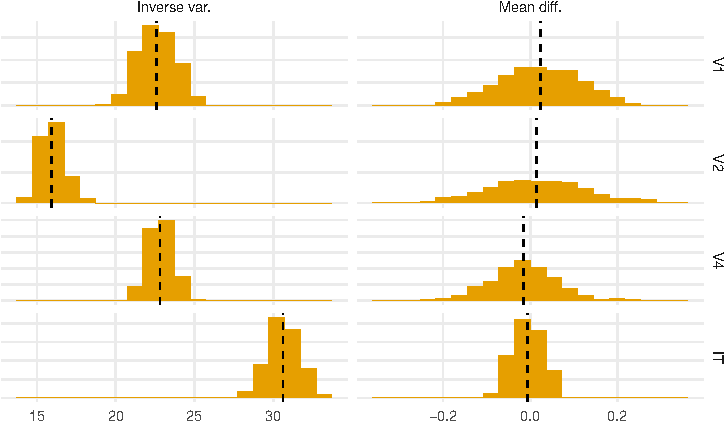
\includegraphics[keepaspectratio]{20260812_files/figure-pdf/fig-dM_mu_var-1.pdf}}

}

\caption{\label{fig-dM_mu_var}Histogram of the average mean difference
and average of the diagonal of the inverse covariance matrix with 40
sites. Trends are similar for 10, 20, and 30 sites (not shown). Results
are taken from the ordinary (no shrinkage) covariance estimator.}

\end{figure}%

\subsection{Between sample
comparisons}\label{between-sample-comparisons}

With only six samples, the inverse covariance matrix needs to be found
with a shrinkage estimator, such as the one provided by
\texttt{corpcor::invcov.shrink()}, which implements the Ledoit-Wolf
shrinkage estimator. When the distances are aggregated over families,
the pairwise distances tend to be largest for V2, a trend that seems to
be consistent when the values are separated by families
(Figure~\ref{fig-pairwise_dM}). This is somewhat inconsistent with
Ziemba et al.'s results, which found that samples were better separated
in V1.

\begin{figure}

\centering{

\pandocbounded{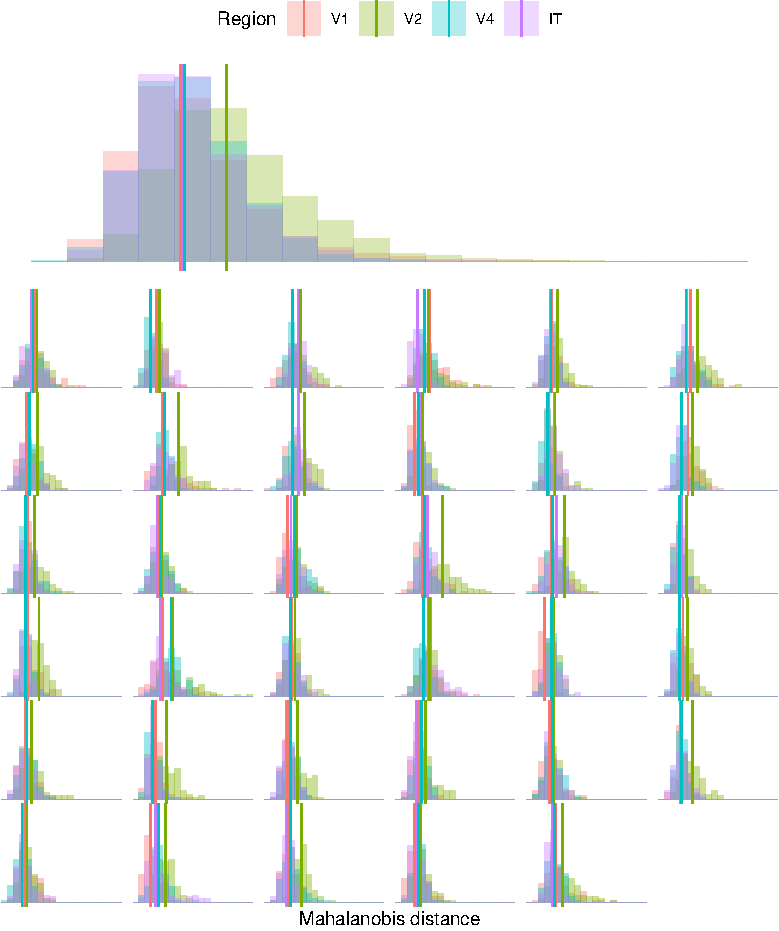
\includegraphics[keepaspectratio]{20260812_files/figure-pdf/fig-pairwise_dM-1.pdf}}

}

\caption{\label{fig-pairwise_dM}Histogram of Mahalanobis distances for
each pairwise sample comparison, either aggregated across all families
(top) or separated by family (bottom) and with fill color based on
region. Vertical lines indicate medians. Note that pairwise distances
must be found with the shrinkage estimator.}

\end{figure}%

The randomized dichotomy results, in order of increasing median
distance, tends to follow V1 \textless{} IT \textless{} V4 \textless{}
V2, which is also not consistent with the previous results in Ziemba et
al.~(2016). Results will be reported with the shrinkage estimator. The
number of sites used does not change the overall pattern of the
distances, but more sites tends to increase the range of calculated
distance values (Figure~\ref{fig-dM_infam}). This does not change with
the ordinary (non-shrinkage) estimator (not shown). I have not yet
analyzed the difference in means and \(\Sigma^{-1}\) for the randomized
dichotomies.

\begin{figure}

\centering{

\pandocbounded{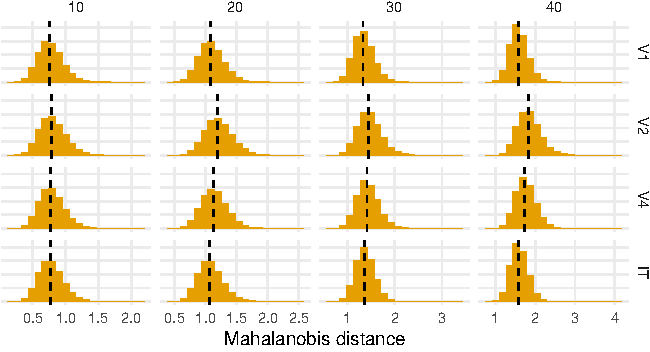
\includegraphics[keepaspectratio]{20260812_files/figure-pdf/fig-dM_infam-1.pdf}}

}

\caption{\label{fig-dM_infam}Histogram of Mahalanobis distances with
different numbers of sampled sites. Results are taken from the shrinkage
inverse covariance estimator.}

\end{figure}%

\section{Next steps}\label{next-steps}

I want to check if z-scoring MUAs affects the trends seen in the
between-family and between-sample comparisons. Then, I want to change my
exploratory procedure to save the entire \(\Sigma^{-1}\) matrix and
check the covariance between sites within each region. Mostly, I do not
have a good intuition for how potential sparsity in V4 and IT may affect
the comparisons, especially if sparsity is not universal. E.g., for each
between-family comparison, the activity of a few sites separates the
families well, but the sites may differ depending on the families being
compared. I am not sure z-scoring will help with this exact question,
though inconsistency between the current analyses and the z-scored
analyses will probably indicate some interesting feature of the
covariance between sites.

The between-sample (within-family) results being inconsistent with
Ziemba et al.~needs to be explained. Ziemba et al.~drew their
conclusions with multi-level ANOVA (decomposing variance into a
between-family, between-sample, and between-repetition component) and
Poisson regression. Possibly, if there is overall higher variance in V2
firing, the scaling of the \(d_M\) comparisons may not ``normalized''
compared to ANOVA. However, it is unclear to me why \(d_M\) would differ
from Poisson regression results.

Furthermore, it might be prudent to consider holding out arrays from V4
and IT. It is likely not possible for V1 and V2, though future analyses
may be performed on the Ziemba et al.~data.

\section{References}\label{references}

\phantomsection\label{refs}
\begin{CSLReferences}{0}{1}
\bibitem[\citeproctext]{ref-portilla_parametric_2000}
\CSLLeftMargin{1. }%
\CSLRightInline{Javier Portilla, Eero P. Simoncelli. A parametric
texture model based on joint statistics of complex wavelet coefficients.
International Journal of Computer Vision. 2000 Oct 1;40(1):49--70.
doi:\href{https://doi.org/10.1023/A:1026553619983}{10.1023/A:1026553619983}}

\bibitem[\citeproctext]{ref-freeman_functional_2013}
\CSLLeftMargin{2. }%
\CSLRightInline{Jeremy Freeman, Corey M. Ziemba, David J. Heeger, Eero
P. Simoncelli, J. Anthony Movshon. A functional and perceptual signature
of the second visual area in primates. Nat Neurosci. 2013
Jul;16(7):974--81.
doi:\href{https://doi.org/10.1038/nn.3402}{10.1038/nn.3402}}

\bibitem[\citeproctext]{ref-lee_developmentally_2024}
\CSLLeftMargin{3. }%
\CSLRightInline{Gerick M. Lee, C. L. Rodríguez Deliz, Brittany N.
Bushnell, Najib J. Majaj, J. Anthony Movshon, Lynne Kiorpes.
Developmentally stable representations of naturalistic image structure
in macaque visual cortex. Cell Reports. 2024 Aug 27;43(8).
doi:\href{https://doi.org/10.1016/j.celrep.2024.114534}{10.1016/j.celrep.2024.114534}}

\bibitem[\citeproctext]{ref-ziemba_selectivity_2016}
\CSLLeftMargin{4. }%
\CSLRightInline{Corey M. Ziemba, Jeremy Freeman, J. Anthony Movshon,
Eero P. Simoncelli. Selectivity and tolerance for visual texture in
macaque V2. Proc Natl Acad Sci USA. 2016 May 31;113(22).
doi:\href{https://doi.org/10.1073/pnas.1510847113}{10.1073/pnas.1510847113}}

\end{CSLReferences}




\end{document}
